
\section*{Problema P6.39}

\renewcommand*\thesection{6.39}
\numberwithin{equation}{section}

\begin{center}
    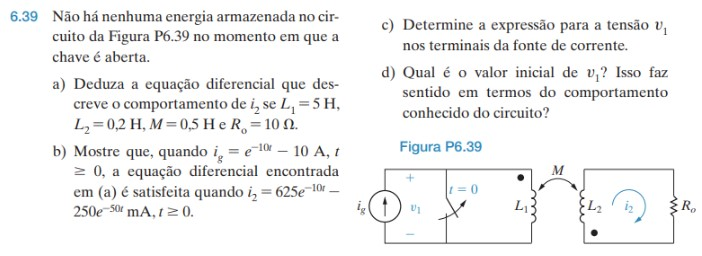
\includegraphics[scale=1.0]{P6.39.jpg}
\end{center}

\subsection*{(a)}

Aplicando análise de malhas no circuito, temos na malha 1:

\begin{equation}\label{eq:6.39.1}
    -v_1(t) + L_1\diff{i_g}{t} + M\diff{i_2}{t} = 0
\end{equation}

Na malha 2,

\begin{equation}\label{eq:6.39.2}
    +i_2R_o + L_2\diff{i_2}{t} + M\diff{i_g}{t} = 0
\end{equation}

Substituindo os valores do enunciado na equação da malha 2,

\[ 10i_2 + 0.2\diff{i_2}{t} + 0.5\diff{i_g}{t} = 0 \]

Isolando $i_2$ na EDO, 

\[ \boxed{0.2\diff{i_2}{t} + 10i_2 = - 0.5\diff{i_g}{t} \quad , \quad t \geq 0}  \]

\subsection*{(b)}

Substituindo o valor fornecido de $i_g(t) = e^{-10t} - 10 \un{A} $ na EDO do item (a), temos

\[ 0.2\diff{i_2}{t} + 10i_2 = (-0.5) (-10e^{-10t}) \]

\[ \diff{i_2}{t} + 50i_2 = 25e^{-10t} \]

A EDO possui fator integrante $M(t)$ dado por 

\[ M(t) = e^{\int 50 \,dt} \logo M(t) = e^{50t} \]

Multiplicando a EDO por $M(t)$,

\[ e^{50t}\diff{i_2}{t} + 50i_2e^{50t} =  25e^{-10t}e^{50t} \]

\[ e^{50t}\diff{i_2}{t} + 50e^{50t}i_2 =  25e^{40t} \]

Aplicando o inverso da regra da derivada do produto,

\[ \diff{\left[i_2 \cdot e^{50t}\right]}{t} = 25e^{40t} \]

Portanto,

\[ i_2 \cdot e^{50t} = \int 25e^{40t} \, dt \]

\[ i_2 \cdot e^{50t} = 25 \frac{1}{40} (e^{40t} + C) \]

\[ i_2 = 0.625 \frac{e^{40t}}{e^{50t}} + \frac{C}{e^{50t}} \]

Finalmente, a solução geral da EDO é

\[ \boxed{i_2(t) = 0.625e^{-10t} + Ce^{-50t} \un{A} \quad , \quad t \geq 0}  \]

Como $i_2(t) = 625e^{-10t} - 250e^{-50t} \un{mA}$ é da mesma forma que a solução geral da EDO, temos que ela satisfaz a
EDO do item (a).

\subsection*{(c)}

A partir de \eqref{eq:6.39.1}, temos

\[ v_1(t) = L_1\diff{i_g}{t} + M\diff{i_2}{t} \]

Usando $L_1 = 5\un{H}$, $M = 0.5 \un{H}$, $i_g(t) = e^{-10t} - 10 \un{A}$ e $i_2(t) = 625e^{-10t} - 250e^{-50t} \un{mA}$, temos

\[ v_1(t) = -50e^{-10t} -3.125e^{-10t} + 6.25e^{-50t} \]

\[ \boxed{v_1(t) = -53.125e^{-10t} + 6.25e^{-50t} \un{V} \quad , \quad t \geq 0}  \]

\subsection*{(d)}

Usando a expressão de $v_1(t)$ calculada no item (c), temos

\[ v_1(0) = -53.125e^{0} + 6.25e^{0} \un{V} \]

\[ \boxed{v_1(0) = -46.875 \un{V}}  \]






